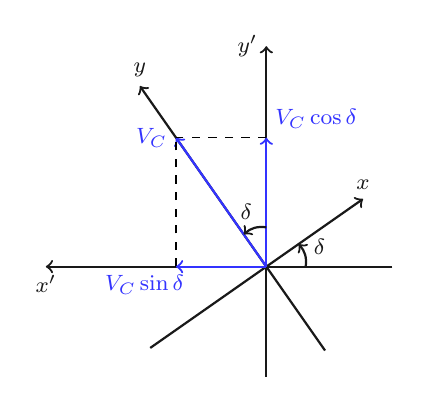
\begin{tikzpicture}
  \begin{scope}
    \footnotesize
    \draw[->,thick,black!90] (1.6,0) -- (-2.8,0)  node[below] {$x'$};
    \draw[->,thick,black!90] (0,-1.4) -- (0,2.8) node[left] {$y'$};
    \draw[->,thick,rotate=35,black!90] (-1.8,0) -- (1.5,0) node[above] {$x$};
    \draw[->,thick,rotate=35,black!90] (0,-1.3) -- (0,2.8) node[above] {$y$};

    \draw[->,thick,blue!80,rotate=35] (0,0) -- (0,2) coordinate(Va) node[left] {$V_C$};
    \draw[-,dashed] (0,{2*cos(35)}) -- (Va);
    \draw[->,thick,blue!80] (0,0) -- (0,{2*cos(35)}) node[above right] {$V_C\cos\delta$};
    \draw[-,dashed] ({-2*sin(35)},0) -- (Va);
    \draw[->,thick,blue!80] (0,0) -- ({-2*sin(35)},0) node[below,xshift=-4mm] {$V_C\sin\delta$};

    \path[->,thick,black!90] (0,.5) edge [bend right=25] node[above,xshift=-1mm] {$\delta$} ({-.5*sin(35)},{.5*cos(35)});
    \path[->,thick,black!90] (.5,0) edge [bend right=25] node[right,yshift=1mm] {$\delta$} ({.5*cos(35)},{.5*sin(35)});
  \end{scope}
\end{tikzpicture}